\documentclass[]{beamer}
\usepackage{easy-pres}
\usepackage[headerslides]{umnbeamertheme}
\usepackage{umnparticles}
\graphicspath{{../common/}}

\newcommand{\commonfiles}[1]{../common/#1}

\title[Subgroup Update]{SUS-RPV Subgroup Update}
\subtitle{Run2+3 Data/MC and Trigger Efficiency Studies}
\date[2025/01/24]{2025/01/24}

\author[Charlie Kapsiak (UMN Single Stop Group) ]{
  Nadja Strobbe\inst{1} \and
  Devin Mahon\inst{1} \and
  \underline{Charlie Kapsiak}\inst{1} \and
  Shardul Rao\inst{1} \and
  Seth Bendigo\inst{1}
}


\begin{document}

\maketitle

\section{Introduction}
\label{sec:introduction}

\begin{frame}{Analysis Target}
  \begin{itemize}
  \item Searching for the production and decay of a single \stop{} to 4 standard model quarks through an RPV coupling. 
  \item Targeting both $\lambda_{312}'',\lambda_{313}'' \in [0.1,0.4]$.
    \begin{itemize}
    \item Intermediate values between long lived ($\lambda < 0.1$) and direct dijet decays ($\lambda > 0.4$)
    \end{itemize}
  \item Well motivated channel to look for SUSY \cite{evans_lhc_2013}:
    \begin{itemize}
    \item Unexplored region of RPV parameter space
    \item Large cross section allows us to probe higher masses
    \end{itemize}
  \item For more information see \href{https://indico.cern.ch/event/1324384/\#2-rpv-single-top-squark-analys}{2023-10-06: Introduction Talk}
  \end{itemize}

  \begin{center}
    %\graphiccite{figures/xsec.png}{0.5}{rasmussen_gaussian_2006}\hspace{1em}
    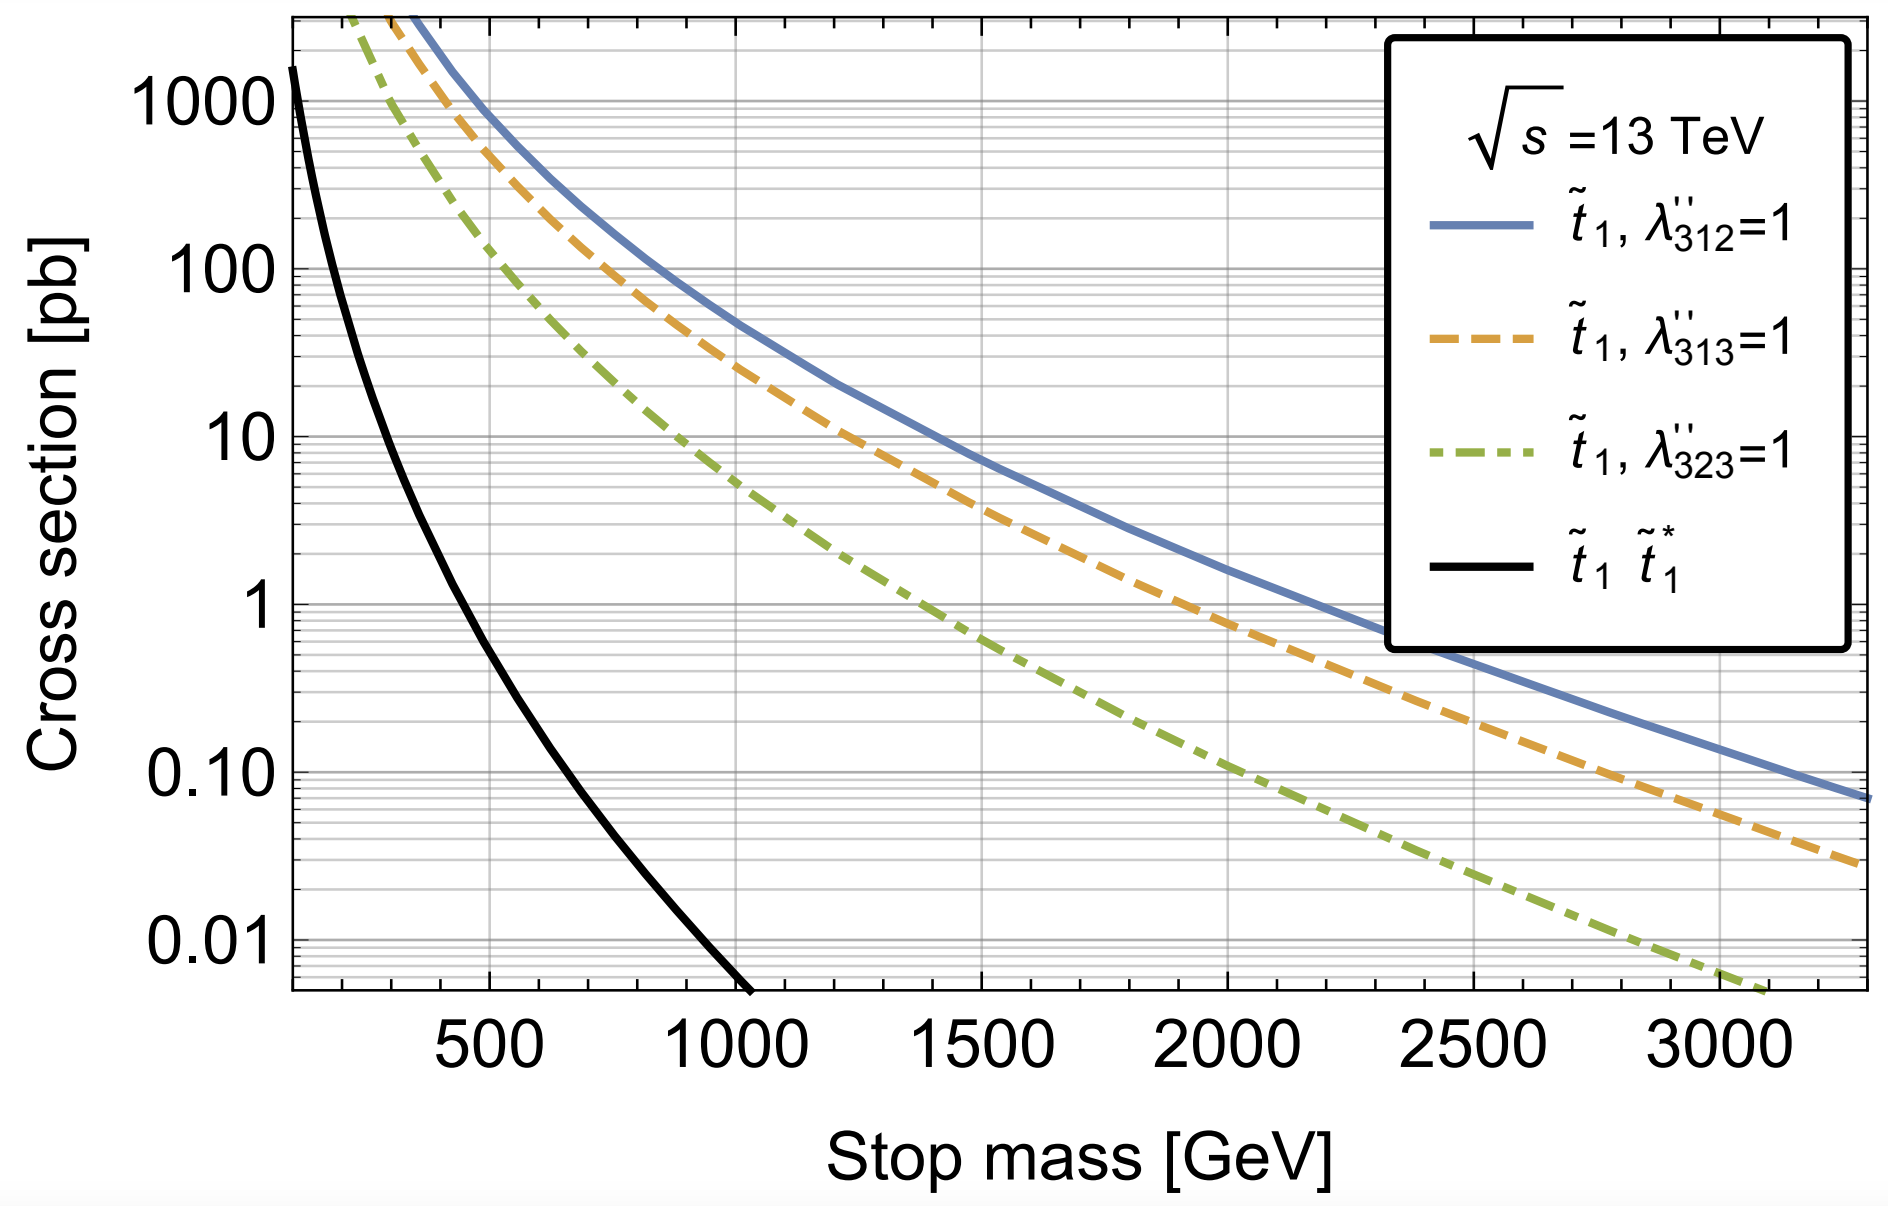
\includegraphics[width=0.5\textwidth]{figures/xsec.png}
    % \scalebox{0.7}{\includestandalone{\commonfiles{general/single_stop}}}
  \end{center}
\end{frame}


\newcommand{\specialcell}[2][c]{\begin{tabular}[#1]{@{}c@{}}#2\end{tabular}}
\begin{frame}[label=regions]{General Analysis Features}
  \begin{itemize}
  \item No leptons.
  \item A moderate number of jets, several with high $p_{T}$.
  \item Multiple b-jets with large angular separation.
  \item Resonances from both the $\stop$ and the $\chinopm$.
  \end{itemize}

  \begin{center}
    \scalebox{0.75}{
      \begin{tabular}{|ccccc|}
        \hline
        \multicolumn{5}{|c|}{Baseline Selections} \\ \hline
        \multicolumn{5}{|c|}{\texttt{HLT\_PFHT* | HLT\_AK8PFJet*\_TrimMass*}} \\
        \multicolumn{5}{|c|}{$4 \leq \mathrm{N_j} \leq 6$ ($p_{\mathrm{T,j}} > 30~\text{GeV}$, $|\eta_{\mathrm{j}}| < 2.4$)} \\
        \multicolumn{5}{|c|}{$p_{\mathrm{T,j_1}} > 300~\text{GeV}$} \\
        \multicolumn{5}{|c|}{$\mathrm{N}_e (\text{tight}), \mathrm{N}_\mu (\text{medium})  = 0$} \\
        \multicolumn{5}{|c|}{\rule[-0.5em]{0em}{0em}$m_4 \equiv m_{\mathrm{j_1,j_2,j_3,j_4}}$} \\ \hline
        \rule{0em}{1.4em}\specialcell{$\lambda_{312}''$\\ Uncompressed SR}
        & \specialcell{$\lambda_{312}''$\\ Compressed SR}
        & \specialcell{$\lambda_{313}''$\\ Uncompressed SR}
        & \specialcell{$\lambda_{313}''$\\ Compressed SR}
        & \specialcell{Control Region} \\ \hline
        $\mathrm{N_{b,M} } \geq 2$ & $\mathrm{N_{b,M} } \geq 2$ & $\mathrm{N_{b,T} } \geq 3$ & $\mathrm{N_{b,M}}  \geq 3$ & $\mathrm{N_{b,L}} = 0$ \\
        $\mathrm{N_{b,T} } \geq 1$ & $\mathrm{N_{b,T} } \geq 1$ &  & & \\
        $\Delta R_{b_{1},b_{2}} > 1$ & $\Delta R_{b_{1},b_{2}} > 1$ & $\Delta R_{b_{1},b_{2}} > 1$ & $\Delta R_{b_{1},b_{2}} > 1$ &  \\
        \rule[-0.5em]{0em}{0em}$m_3 \equiv m_{\mathrm{j_2,j_3,j_4}}$ & $m_3 \equiv m_{\mathrm{j_1,j_2,j_3}}$ & $m_3 \equiv m_{\mathrm{j_2,j_3,j_4}}$ & $m_3 \equiv m_{\mathrm{j_1,j_2,j_3}}$ & {} \\
        \hline
      \end{tabular}
    }
    
  \end{center}
\end{frame}


\section{Trigger Efficiencies}
\label{sec:trigger-efficiencies}

\begin{frame}{Description}
  
\end{frame}


\section{Data/MC Comparisons}
\label{sec:datamc-comparisons-1}


\section[Significance]{Preliminary Significance Studies}
\label{sec:prel-sign-stud}

\section{Conclusion}
\label{sec:conclusion}




\end{document}





% Local Variables:
% eval: (progn (setq process-environment (copy-sequence process-environment))
% (let* ( (basedir (file-name-directory (directory-file-name (file-name-directory (buffer-file-name)))))
% (texmfpath (file-name-concat  basedir "tex-styles"))
% )
% (setq-local TeX-style-path (append TeX-style-path  (directory-files-recursively texmfpath "auto" t)))
% (setq-local reftex-bib-path (list basedir))
% (setenv "TEXINPUTS" (format "%s:" texmfpath ))
% (setenv "BIBINPUTS" basedir ))
% )
% End:
